\documentclass[authoryear]{book}
\pdfoutput=1


\usepackage{graphics}
% or use the graphicx package for more complicated commands
\usepackage{graphicx}
\usepackage{makeidx}
\usepackage{pgf}
\usepackage{epsfig}
\usepackage{amssymb}
\usepackage{amsmath,latexsym}
\usepackage{array}
\usepackage[round]{natbib}
\usepackage{subfigure}
\usepackage{amsthm} %For theorems
 \usepackage{url}
 \usepackage{ifpdf}


\newcommand{\bm}[1]{\mbox{\boldmath $#1$}}

\makeindex

\theoremstyle{definition}
\newtheorem{theorem}{Theorem} %? [section]
\newtheorem{definition}[theorem]{Definition}
\newtheorem{question}{Question}
\newtheorem{answer}{Answer}


%\usepackage{Sweave}   
\usepackage{setspace} 
\setlength{\parindent}{0cm} 

\headsep=50pt
%\setlength{\parskip}{1.2ex}
\setlength{\parindent}{0.0mm}
\setlength{\textwidth}{16.5cm}
\setlength{\textheight}{23cm}
\setlength{\hoffset}{-0.8in}
\setlength{\voffset}{-1.3in}
\linespread{1.05}

\parindent=1.5pc
%\parskip=0pt
\setcounter{section}{0}
%\setcounter{tocdepth}{0}
% \setcounter{secnumdepth}{3}
%\textwidth=33pc
%\textheight=50pc
%\renewcommand{\figurename}{Fig.}

\def\Prob{\text{Prob}}
\def\E{\text{E}}
\def\Cov{\text{Cov}}
\def\Corr{\text{CoRrr}}
\def\Var{\text{Var}}
\def\Prec{\text{Prec}}
\def\R{\mathbb{R}}
\def\S{\mathbb{S}}


\def\mm#1{\ensuremath{\boldsymbol{#1}}} % version: amsmath
\def\MyFigureWidth{0.4\textwidth}
\def\MyFigureWidthTwo{9.5cm} %% 2*width + spacing
\def\MyFigureSpacing{6mm}

%%  To change the page layout from the default
%\addtolength{\topmargin}{-2cm}
%\addtolength{\textheight}{3cm}
%\addtolength{\oddsidemargin}{-0.5cm}
%\addtolength{\textwidth}{1cm}

% \SweaveOpts{width = 40}

\setkeys{Gin}{width=0.45\textwidth}

%\definecolor{links}{HTML}{2A1B81}
%\hypersetup{colorlinks,linkcolor=,urlcolor=links}

\def\SHS#1{\textcolor{blue}{SHS: #1}}
\def\JBI#1{\textcolor{green}{JBI: #1}}
\def\DB#1{\textcolor{red}{\textbf{DB: #1}}}

\title{Flexible spatial modelling with INLA and inlabru}

\author{Janine B Illian and others }

\date{\today}

\setcounter{chapter}{0}
\begin{document}
\maketitle

\graphicspath{{./figures/chap_1/}}

\chapter{The key ideas}

% Not too long, so that it can be read quickly

\section{Introduction -- what is this book about}
Somebody who opens this book might wonder -- it this book for me? What is this book about and will I benefit from reading it?
 Many of you might have heard about INLA and have picked this book up because it has INLA in the title-- and can teach you ``How to use INLA'' or what models can be fitted with. Others might have come across this book they are familiar with INLA, but would like to see a wide  range of models that may be fitted with INLA. The things is-- this book is not about INLA.
 
In this first chapter we illustrate what this book  is about, by showing examples of a number of data structures that may be seen a typical special cases that the analysis methods discussed in this book can deal with. When reading this you may find that some of the data sets initially seem to be very different in structure. In this chapter we show the diversity and pointing out similarity.

INLA is a model fitting method -- we will discuss it in detail below -- and as such a means to an end. 
Spatial component that has not been traditionally pointed out/discussed.


\section{Examples -- data structures}

Lets have a look at a few examples of data structures.

\subsection{Spatially continuous data}
% to do:
% find appropriate data set

Consider Figure \ref{fig:elev} which shows the elevation in a rainforest study plot in Panama. In this data structure that  takes on values everywhere in the plot; there is not a single location where it would not make sense to consider elevation as the quantity is spatially continuous.
\begin{figure}
\centering
%\includegraphics[width=0.3\textwidth]{complete}
%\includegraphics[width=0.6\textwidth]{sealsscotland}
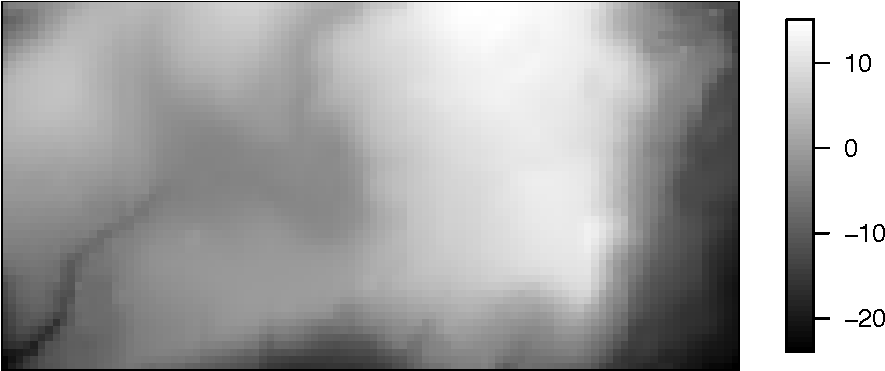
\includegraphics[width=0.6\textwidth]{elev}
\caption{\label{fig:elev} Some elevation somewhere...}
\end{figure}
In practice, however, there are limitations. While there are there are infinitely many locations in even a small area of space the quantity of interest cannot be measured everywhere in space -- and the quantity of interest cannot be fully observed. It can only be measured at a finite number of locations and these location have typically been chosen as part of the study design. There is an interest in interpolating to locations where no measurements have been taken -- referred to as \textit{spatial prediction}. This prediction into other areas of space needs to be done in a clever way, that take into account information from given measurements. In particular, on would like the predicted values to be similar to the values measured in the other locations. The figure is actually based on XX measurements in as many locations randomly distributed across the plot. There might also be an interest in relate one spatially continuous variable to other spatially continuous variables as part of a modelling exercise. These spatial covariates might help to explaining why values are high/low in different areas of the plot, but there might still be spatial structure left that needs to be accounted for.

This data structure is often referred to as \textit{geo-referenced data}\index{geo-referenced data} or \textit{geostatistical data}\index{geostatistical data}.

\subsection{Spatial point patterns}
Figure \ref{fig:rainpattern} shows  the same rainforest study plot as Figure \ref{fig:elev}, but this time the locations of trees of the species \textit{Beilschmidia} have been plotted. A study might be interested in analysing the pattern formed by those trees to understand habitat preferences of the species. Hence, unlike in the previous example the locations have not been deliberately chosen as part of the study but are the object of interest. The main interest is to understand-- and hence model the spatial pattern.
Again, spatial covariates might explain the spatial pattern but there might still be spatial structure left that needs to be accounted for.

This data structure is referred to as a \textit{spatial point pattern}\index{spatial point pattern}.
\begin{figure}
\centering
%\includegraphics[width=0.3\textwidth]{complete}
%\includegraphics[width=0.6\textwidth]{sealsscotland}
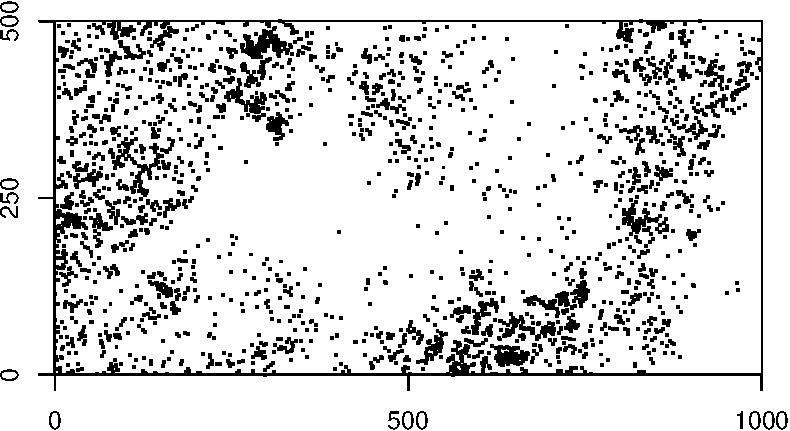
\includegraphics[width=0.6\textwidth]{rain_pattern}
\caption{\label{fig:rainpattern} Rainforest trees...}
\end{figure}




\subsection{Data collected on transects}
\subsection{Distance sampling data}


\section{Synergy -- common spatial structure}
Datasets collected in different ways -- but the all have 
a spatial structure. Spatial structure is relevant, of interest or might impact on inference.

How do we represent this spatial structure? This is how 

\subsection{The random field -- intuition}



\subsection{Issues with spatial data analysis}

Computationally complex. Hence need to be computationally efficient.

Need to approximate.

Space is complex (sphere, holes) -- need to be flexible. Grids are rigid... 

\section{What to expect from the book}


Finding a rigorous yet flexible way of representing the spatial structure and linking this with computationally efficient model fitting strategies that allow us to fit relevant and realistically complex models.

\section{Structure of the book}

Next Chapter explores key concepts by referring to the different data structures we have seen here. It ends with a roadmap of this book.
 
Chapter after that formalises these concepts




\graphicspath{{./figures/chap_2/}}
\chapter{Key concept--spatial point processes}


\section{A spatial point pattern}
% kleines Beispiel durchziehen
%David's data

Refer to Figure \ref{fig:rainpattern2}, which shows the spatial pattern formed by rainforest trees in a tropical rainforest in XXX. 

\begin{figure}
\centering
%\includegraphics[width=0.3\textwidth]{complete}
%\includegraphics[width=0.6\textwidth]{sealsscotland}
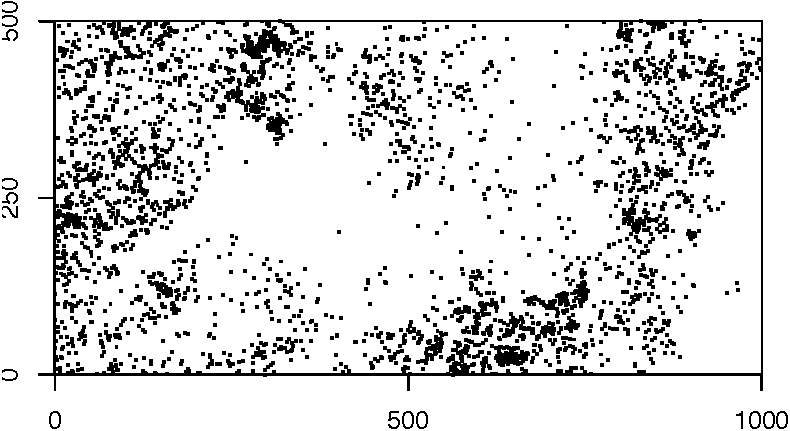
\includegraphics[width=0.6\textwidth]{rain_pattern}
\caption{\label{fig:rainpattern2} Rainforest trees...}
\end{figure}

It has some structure to it -- there are areas where we find more trees than in other areas, i.e.\ the density of trees varies in space. There is an interest in understanding why this is the case- and hence a study aim could be to understand the spatial structure formed by the locations of trees in space.
This is what point processes do -- they describe and model the spatial structure of 
 
\section{Spatial point processes--intuition}
Model location of objects in space.

\subsection{The intensity}
Initially one might want to understand how the density of trees varies in space, i.e.\ get a quantitative description of the number of individuals in space.

\subsection{Relationship to covariates}

\subsection{}


\section{Thinned point processes}

\subsection{Known thinning process}

\subsection{Unknown thinning process}

\section{Spatial point processes-- technical}
\subsection{Mathematical background}\label{ch1_maths}
The methodology developed for spatial point pattern data seeks to describe and analyse the patterns to infer information on the underlying mechanisms that generated them, i.e., a \textbf{spatial point pattern} formed by the spatial locations of objects in $d$-dimensional space, i.e.\ $\mathbf{x}=(x_1, \ldots, x_n)$, where $x_i \in \R^d, i = 1, \ldots, n$ and we typically have $d = 2$ or $d = 3$. 

%\janine{examples of patterns - properties -- thesis}

Technically, a spatial pattern is regarded as a realisation from a \textbf{random variable}, i.e.\  a stochastic structure that follows some distribution, referred to as a \textbf{spatial point process} $\mathbf{X}$. To understand this, recall the perhaps more familiar situation of data that are considered realisations from a theoretical random variable (or model) that follows, e.g., a normal distribution. In the context of spatial point patterns, the situation is complicated by the fact that all the points in the pattern together and the constellation that they form is a single observation (a single ``datum"). This implies that the random variable describing such a structure is bound to be a complicated mathematical object and hence to follow a rather complex distribution. This also implies that if an analysis is concerned with a single point pattern all information on this distribution has to be extracted from a single realisation\footnote{Ergodicity.}.

In this book, we focus on the practical analysis of spatial point patterns and refer the reader interested in the mathematical  details underlying spatial point processes to the relevant statistical literature.  However, to appreciate that a point pattern differs from a standard dataset and that it is indeed a complicated object note that a suitable random variable representing this data structure needs to capture the fact that the number of observed points is random. This implies that the mathematically complicated concept of a random measure has to be used. This in turn means that even the mathematics underlying a model for a data set with relatively simple structure such as the one in Figure \ref{chap1:fig1} are challenging. It is hence not surprising that within the history of mathematics these models have been described only relatively recently. Outside the statistical literature they have been considered very rarely but are becoming more popular these days.

A probability distribution (or model) familiar from non-spatial statistics assigns different probabilities to different realisations of a random variable -- realisations from a normal distribution are more likely to take on values that are close to the mean value but are less likely to take on values that are very different from the mean.  
Similarly, a specific \textbf{spatial point process model} characterises the properties of the random variable by assigning different probabilities to different realisations of the point process, only that now the realisations are point patterns. For instance, realisations from a model that reflects clustering are likely to be clustered and rather unlikely to be regular.  To achieve this, the mathematical formulation of a spatial point process model contains parameters.  These reflect the characteristics of the process and ultimately the characteristics of the generated patterns, i.e.\ characteristics such as clustering, regularity or randomness as well as homogeneity or inhomogeneity.  A number of different \textbf{classes} of spatial point process models with similar mathematical descriptions and properties have been formulated in the literature (see e.g.\ \cite{lieshout:00}, \cite{moeller:03}, \cite{stoystoy:94}).






\graphicspath{{./figures/chap_3/}}
\chapter{The key concept--Gaussian random field}

\section{Introduction -- random fields, a gentle introduction}
We have seen in the first chapter that many data structures have one thing in common--they life in space where there is spatial autocorrelation. This autocorrelation is reflected in a random field.

A spatial random field is a \textit{random variable}\index{random variable} that represents spatially continuous phenomena in 2 dimensions. Since this is a difficult concept to grasp this chapter slowly builds up to these by first considering simple univariate random variables familiar from basic statistics courses, then moving to 1-dimensional random fields and eventually the 2-dimensional random fields that will be prominent throughout this book.


\subsection{A simple univariate random variable}

\textit{Random variables} are a key concept in all statistical literature as they are the basic objects that are used in all statistical inference. Random variables are variables that are assumed to follow some probability distribution, i.e.\ they take on different values or values within a certain interval with different probabilities. 
% something on a discrete random variable
A very familiar example is a random variable that follows a normal distribution. This one-dimensional continuous random variable can take on any value, but values close to the mean are particularly likely, resulting in the famous bell curve. As an example lets assume that IQ values in a country are normally distributed with mean 100 and standard deviation 15. The probability density of this distribution is plotted in Figure \ref{fig:ch2:normal}, black line indicating that values around the mean rather likely and those further away are less likely. 

\begin{figure}
\centering
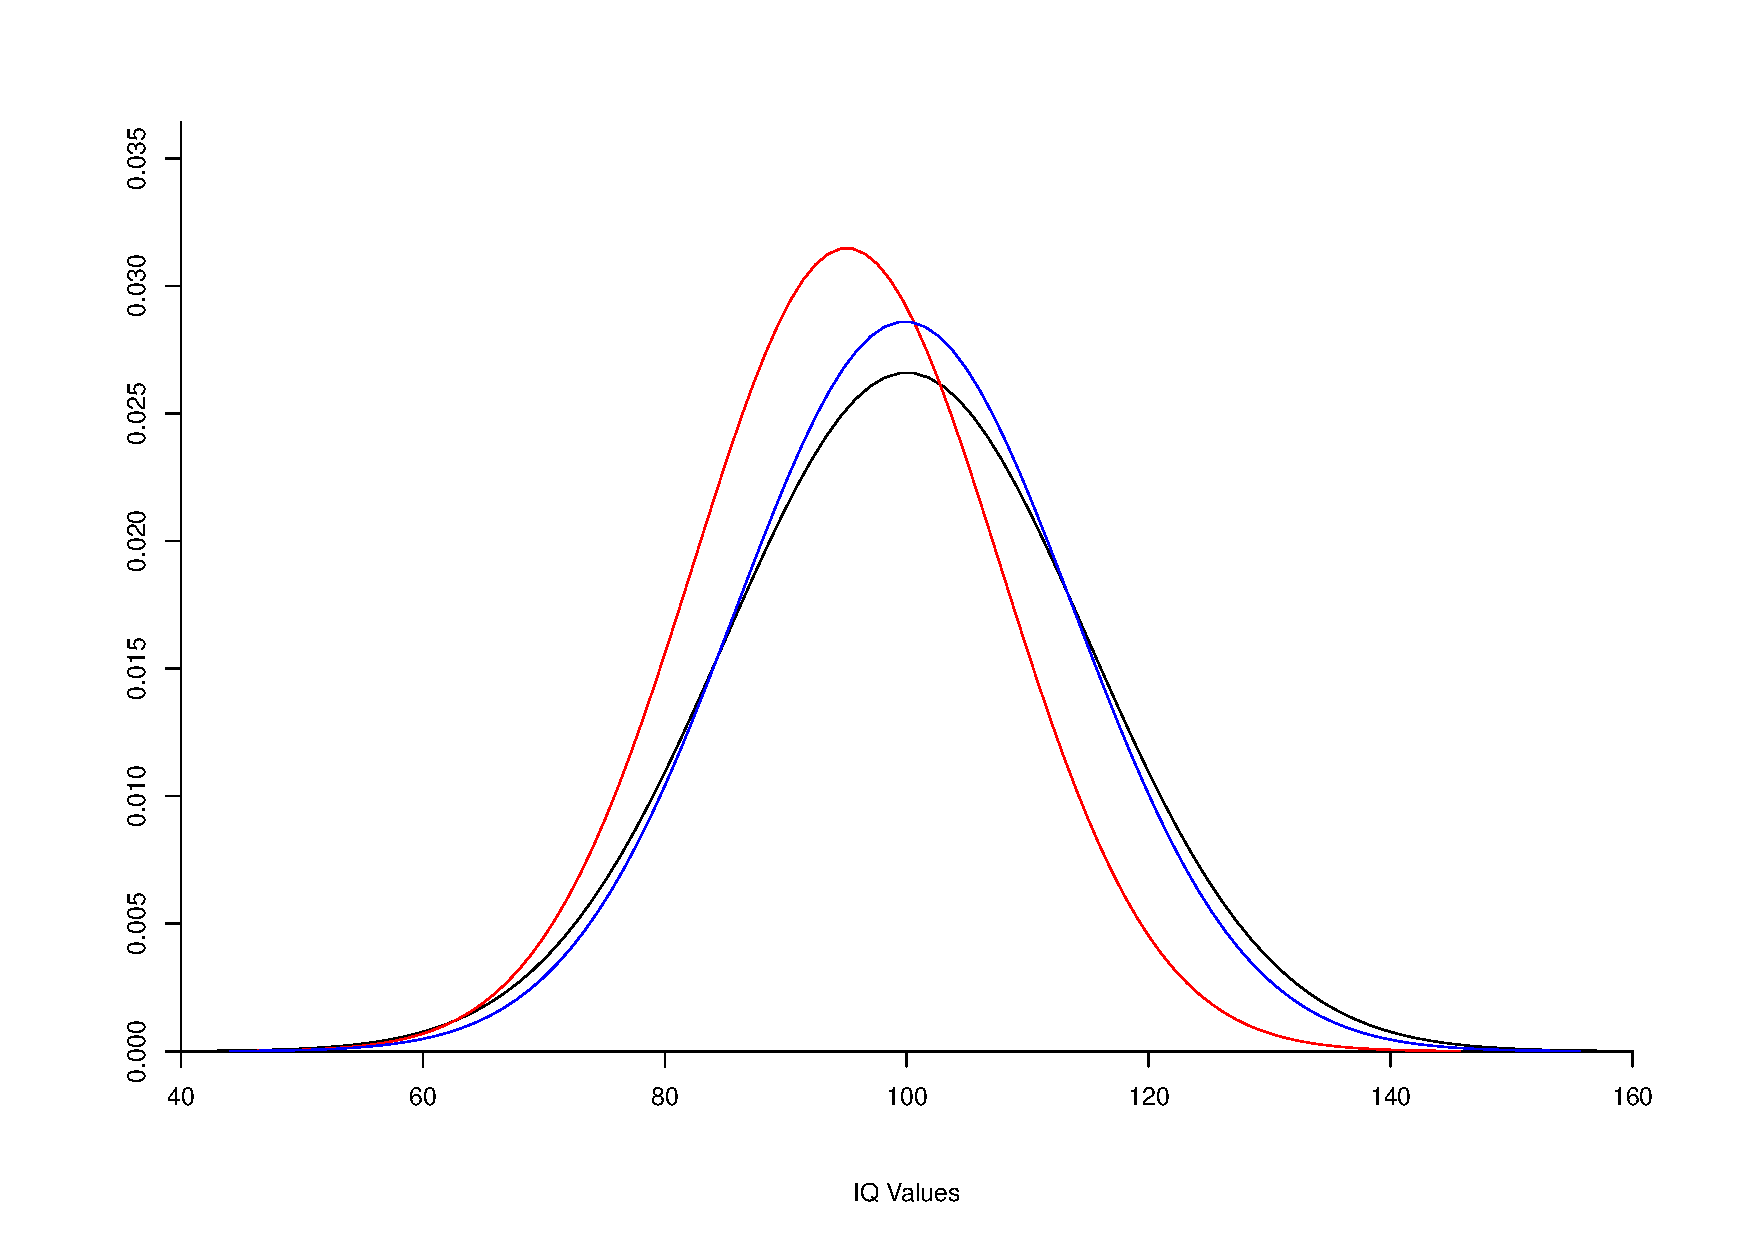
\includegraphics[width=0.5\textwidth]{normal_density}
\caption{\label{fig:ch2:normal} The probability density of the normal distribution with mean 100 and sd = 15 (black line), the density estimated from a sample of size 20 (red line) and the density estimated from a sample of size 200 (blue line). }
\end{figure}

In practice, we usually do not know the true distribution for a given population but use a \textit{sample} to estimate the parameters of the distribution from this sample, for example using maximum likelihood estimation methods, as discussed in standard statistics textbooks. For the example in Figure \ref{fig:ch2:normal} a sample of size 20 resulted in an estimate of mean 95.03 and standard deviation 12.67; the estimated density is shown as the red line in the same figure. However, a much bigger sample of size 200 provided a much better estimate with a mean of 99.84 and standard deviation 13.95, represented by the blue line in Figure \ref{fig:ch2:normal}. This improvement in precision is not surprising as we gain more \textit{independent information} on a population from a sample of a bigger size and hence our estimates become more precise. 

An important point here is that typical estimation and inference approaches assume that any sample consists of \textbf{independent observations} or \textbf{replicates}.  Dependent samples are likely to tend to be similar and hence to not provide much new information on the population. This will eventually introduce bias.  In practical \textit{data collection} independent observations are obtained by making sure that there are no similarities or relationships among any of the observations as a result of the sampling process itself. For instance, for the estimation of IQ values in a country one would have to sample across the population and not just from a specific subgroup  of the population, say university students, as this would bias the estimation. In this case there is a similarity or relationship among the resulting observations as the observation have all be been made from members of the same subgroup.

We will see further below that the central concept of the book--in random fields--there is no assumption of independence among measurements; they are explicitly assumed to show \textbf{systematic dependence} among measurements and a specific  assumption is made about the nature of this dependence. We will start thinking about this dependence in the next section. We will initially look at a one dimensional random field even though most of the random fields discussed in this book are spatial random fields, i.e.\ random fields in 2D.

\subsection{A random field in 1D}
A random field in 1D is a random variable the realisations of which take on values in one-dimensional space. Lets think about this through an example. Say, the 25 children in a primary school class in Helsinki are set to learn about temperature, its measurement and how it fluctuates in their home town during a day in spring. In other words, the random variable of interest is ``temperature throughout school day in spring in Helsinki''.  To estimate this random variable on one specific day in May,  the children are each given a different random time between 8:00 am and 4:00 pm by their teacher and are asked to check and write down the temperature at the thermometer in their classroom that measures the outside temperature at exactly that time. 


When comparing these data to the IQ data we discussed earlier we realise a number of things. Clearly, these temperature measurements are \textit{not independent}--it is likely that the measurements taken at as 12:45 and at 12:50 are not very different from each other. The measurements tell us about the temperature throughout a specific school day in one place in Helsinki, but they do not tell us much about the temperature and its fluctuations elsewhere in the country or the world. Even if each child was given two random times to measure the temperature and the number of observations was doubled, these would not improve our knowledge about the temperature levels and fluctuations that day elsewhere.

However, this is not what the children where meant to learn anyway --they were meant to get a picture of the behaviour of temperature throughout a day in spring in Helsinki. This variable is continuous in time as there is a temperature value associated to any given point in time. However, the children have only measured it at some points in time, not continuously through time -- and it is generally infeasible to do so, as there a infinitely many time points. However, if one makes some general reasonable assumptions as to how temperature behaves over time, it is possible to get an idea of the temperature at times when it has not been measured, based on the given values. 
%Figure \ref{fig:ch2:1D} shows an example of this [bad figure]. 
\begin{figure}
\centering
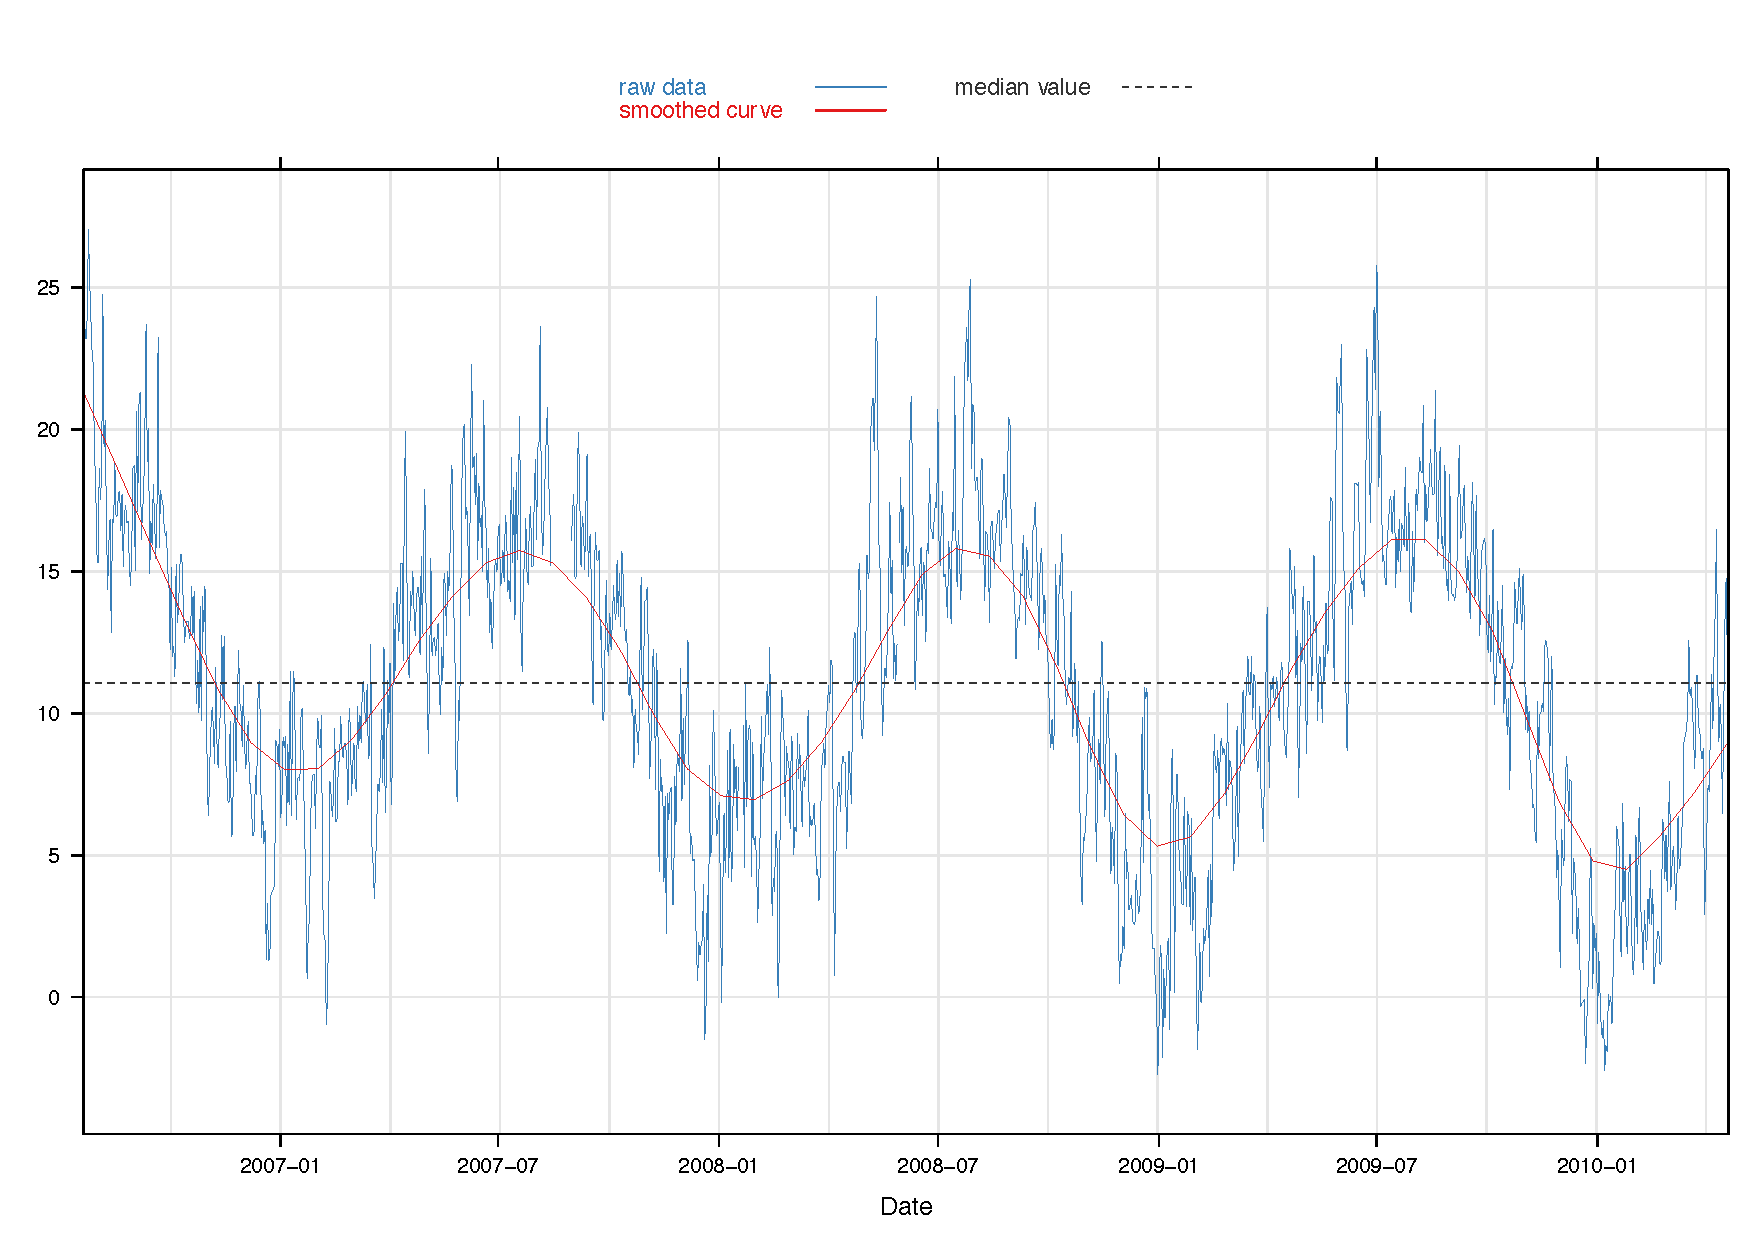
\includegraphics[width=0.5\textwidth]{temp_timeseries}
\caption{\label{fig:ch2:1D} Temperature over time... this is a bad plot....}
\end{figure}
Intuitively, one would want to assume 
\begin{itemize}
\item[a)]  that, on average, same behaviour everywhere and 
\item[b)] that temperature values measured within a few minutes of each other are similar to each other. 
\end{itemize}


We are explicitly assuming that observations are dependent and with the assumptions listed above we implicitly make assumptions about the nature of the dependence among the observations. The fact that two observations in each other's vicinity are similar implies that the temperature does not jump to a different value from one instant to the next; i.e.\ that it varies \textit{smoothly}, and that we can express the dependence through a function of distance between two points
Hence we would like some smooth function to describe the relationship between two observations--and this smooth function depends on distance between the observations and describes their similarity.


%With these simple assumptions one could just  connect the observations by straight line, as in Figure \ref{fig:ch2:1D}; doing this means we are simply taking the average between the values. But we know that temperature does not behave like this and that it is more smooth.

Note that the temperatures in this example have only been observed on one single day, while there is an interest in temperatures in Helsinki in spring. This is implies  that different values would be observed if a different day was chosen. 
%Also, if different times for measuring the 
only one realisation.


While the school children in Helsinki could probably repeat the measurement procedure on several  --randomly chosen-- days throughout spring, in many realistic examples This has important consequences 

Note that measured only at very few points
and this realisation has not been fully observed




Note there is actually another set of assumptions at work here- one that concerns the measuring process.
\begin{itemize}
\item[c)] that temperature is measured at different times during the day and year and month  
\item[d)] and that the person does not get into their car more frequently when it is warmer outside than when it is cold.
\end{itemize}
[example does not work very well; fewer values during the night, but wanted non-regular measurements that one would get from some measurement device...]



\begin{itemize}
\item realise that observations are not independent through time
\item prediction hence needs to take the other values into account 
\item interpolated values should, on average, be similar to all values measured
\item interpolated values should be similar to values measured close in time
\end{itemize}



random field has properties that describe average behaviour and on distance in time


\subsection{The same thing in 2D}
Lets now move to 2 dimensional space.  Temperature again, but now we are interested in measuring in space. Again, we explicitly assume dependence 
Similarity is again expressed through a function that is 

key points:
\begin{itemize}
\item realise that observations are not independent through space
\item interpolated values should, on average, be similar to all values measured
\item interpolated values should be similar values close in space
\end{itemize}

\section{Random fields -- and how they appear everywhere}

Lets have a look at a few examples of data structures.

\subsection{Spatially continuous data as random fields}

\subsection{Spatial point processes, conditional on random fields}

\subsection{Transect data thinned spatial point processes, conditional on random fields}

\section{Random fields -- technical definition}


\graphicspath{{./figures/chap_4/}}
\chapter{Random fields in practice}

\section{Random fields in practice -- approximating a continuous structure}

\subsection{Approximation by a regular grid}
\subsection{Approximation by a triangulation}

\section{Random fields in practice -- computational challenges}
There are computational challenges with random fields.

\subsection{Why are random fields hard to fit?}

\section{INLA}



\section{Outlook}

Chapter on details of INLA ad SPDE approximation can be skipped if technical details not of interest (Sigrunn)

Chapter on mesh construction (Finn!)


\printindex
\end{document}














\chapter{Introduction to book}

\section{Introduction -- what is this book about}
Somebody who opens this book might wonder -- it this book for me? What is this book about and will I benefit from reading it?
 Many of you might have heard about INLA and have picked this book up because it has INLA in the title-- and can teach you ``How to use INLA'' or what models can be fitted with. Others might have come across this book they are familiar with INLA, but would like to see a wide  range of models that may be fitted with INLA. The things is-- this book is not about INLA.
 
In this first chapter we illustrate what this book  is about, by showing examples of a number of data structures that may be seen a typical special cases that the analysis methods discussed in this book can deal with. When reading this you may find that some of the data sets initially seem to be very different in structure. In this chapter we show the diversity and pointing out similarity.

INLA is a model fitting method -- we will discuss it in detail below -- and as such a means to an end. 
Spatial component that has not been traditionally pointed out/discussed.


\section{Examples -- data structures}

Lets have a look at a few examples of data structures.

\subsection{Spatially continuous data}
% to do:
% find appropriate data set

Consider Figure \ref{fig:elev} which shows the elevation in a rainforest study plot in Panama. In this data structure that  takes on values everywhere in the plot; there is not a single location where it would not make sense to consider elevation as the quantity is spatially continuous.
\begin{figure}
\centering
%\includegraphics[width=0.3\textwidth]{complete}
%\includegraphics[width=0.6\textwidth]{sealsscotland}
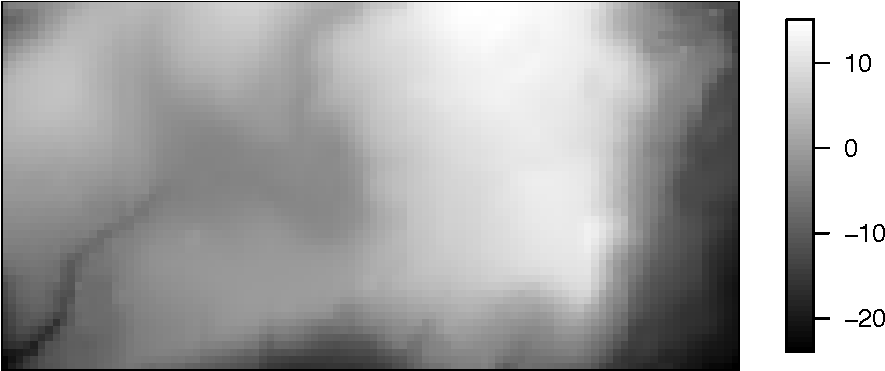
\includegraphics[width=0.6\textwidth]{elev}
\caption{\label{fig:elev} Some elevation somewhere...}
\end{figure}
In practice, however, there are limitations. While there are there are infinitely many locations in even a small area of space the quantity of interest cannot be measured everywhere in space -- and the quantity of interest cannot be fully observed. It can only be measured at a finite number of locations and these location have typically been chosen as part of the study design. There is an interest in interpolating to locations where no measurements have been taken -- referred to as \textit{spatial prediction}. This prediction into other areas of space needs to be done in a clever way, that take into account information from given measurements. In particular, on would like the predicted values to be similar to the values measured in the other locations. The figure is actually based on XX measurements in as many locations randomly distributed across the plot. There might also be an interest in relate one spatially continuous variable to other spatially continuous variables as part of a modelling exercise. These spatial covariates might help to explaining why values are high/low in different areas of the plot, but there might still be spatial structure left that needs to be accounted for.

This data structure is often referred to as \textit{geo-referenced data}\index{geo-referenced data} or \textit{geostatistical data}\index{geostatistical data}.

\subsection{Spatial point patterns}
Figure \ref{fig:pattern} shows  the same rainforest study plot as Figure \ref{fig:elev}, but this time the locations of trees of the species \textit{Beilschmidia} have been plotted. A study might be interested in analysing the pattern formed by those trees to understand habitat preferences of the species. Hence, unlike in the previous example the locations have not been deliberately chosen as part of the study but are the object of interest. The main interest is to understand-- and hence model the spatial pattern.
Again, spatial covariates might explain the spatial pattern but there might still be spatial structure left that needs to be accounted for.

This data structure is referred to as a \textit{spatial point pattern}\index{spatial point pattern}.
\begin{figure}
\centering
%\includegraphics[width=0.3\textwidth]{complete}
%\includegraphics[width=0.6\textwidth]{sealsscotland}
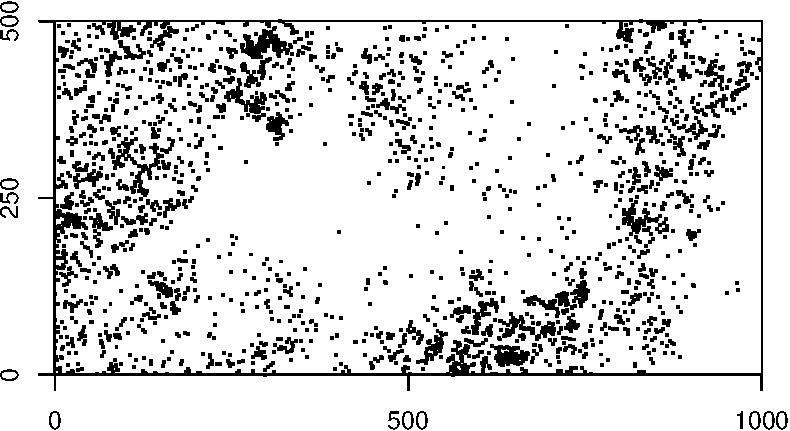
\includegraphics[width=0.6\textwidth]{rain_pattern}
\caption{\label{fig:pattern} Rainforest trees...}
\end{figure}

\subsection{Data collected on transects}
\subsection{Distance sampling data}


\section{Synergy -- common spatial structure}
Datasets collected in different ways -- but the all have 
a spatial structure. Spatial structure is relevant, of interest or might impact on inference.

How do we represent this spatial structure? This is how 

\subsection{The random field -- intuition}



\subsection{Issues with spatial data anlysis}

Computationally complex. Hence need to be computationally efficient.

Need to approximate.

Space is complex (sphere, holes) -- need to be flexible. Grids are rigid... 

\section{What to expect from the book}


Finding a rigorous yet flexible way of representing the spatial structure and linking this with computationally efficient model fitting strategies that allow us to fit relevant and realistically complex models.

\section{Structure of the book}

Next Chapter explores key concepts by referring to the different data structures we have seen here. It ends with a roadmap of this book.
 
Chapter after that formalises these concepts
\printindex

\end{document}



